\documentclass[eng]{mgr}
\usepackage{polski}
\usepackage[utf8]{inputenc}
%\usepackage{xcolor}
\usepackage[T1]{fontenc}

%pakiety do grafiki
\usepackage{graphicx}
\usepackage{psfrag} 

%Wspomaganie tabel
\usepackage{array}
\usepackage{tabularx}
\usepackage{hhline}
%Matematyka
\usepackage{amsmath}
\usepackage{amsfonts}
\usepackage{hyperref}
\usepackage{float}
%pakiet wypisujący na marginesie etykiety równań„ i rysunkóww zdefiniowanych przez \label{}, chcąc wygenerować finalną wersję dokumentu wystarczy usunąć poniższą linię
%\usepackage{showlabels}
%\newcommand{\R}{I\!\!R} %symbol liczb rzeczywistych,
%\newtheorem{theorem}{Twierdzenie}[section] %nowe otoczenie do składania twierdzenia
\usepackage{subcaption}
\usepackage{fancyref}
\title{Zastosowanie sztucznych sieci neuronowych do predykcji wyników meczów tenisa ziemnego}
\engtitle{Artificial neural networks for predicting results of tennis matches}
\author{Szymon Płaneta}
\supervisor{dr inż. Andrzej Rusiecki} 
\field{Automatyka i Robotyka (AIR)}
\specialisation{Technologie Informacyjne \\ w Systemach Automatyki (ART)}

\begin{document}
\maketitle
\tableofcontents

\chapter{Wstęp}

\section{Tenis ziemny}
\label{Sec:Tenis}
Tenis ziemny to jedna z najbardziej popularnych dyscyplin sportowych na świecie. Mecze rozgrywane są pojedynczo (singiel), w dwuosobowych zespołach jednej płci (debel) lub obu płci (mikst). Gra w tenisa w formie jaką mamy dzisiaj wywodzi się z Birmingham w~Anglii. Początki tego sportu datowane są na lata 60. XIX wieku. Najstarszy turniej na świecie, Wimbledon, pierwszy raz odbył się w roku 1877, a w latach 1896-1924 tenis był dyscypliną olimpijską. Na listę dyscyplin olimpijskich został ponownie wpisany w roku 1988 \cite{tenis01}.

W meczu tenisa może wziąć udział każdy, kto jest w stanie trzymać rakietę. Dzięki temu ilość graczy rekreacyjnych można liczyć w milionach. Tenis jest sportem widowiskowym, dlatego zmagania profesjonalistów dostarczają wielu wrażeń i gromadzą liczną widownię. Najbardziej prestiżowymi turniejami w sezonie są cztery turnieje wielkoszlemowe: Australian Open, French Open (znany również jako Roland Garros), Wimbledon oraz US Open. Kolejną rangą turniejów w tenisie męskim są turnieje z cyklu ATP World Tour: ATP World Tour Masters 1000 (cykl dziewięciu turniejów), ATP World Tour 500 i~ATP World Tour 250 \cite{tenis02}.

\begin{table}[H]
\centering
\caption{Turnieje wielkoszlemowe \cite{tenis02}}
\label{Tab:Slam}
\begin{tabular}{|l|l|l|l|}
\hline
\textbf{Data}       & \textbf{Nazwa turnieju}     & \textbf{Miejsce rozgrywek} & \textbf{Nawierzchnia} \\ \hline
Styczeń - Luty      & Australian Open             & Melbourne                  & Twarda                \\ \hline
Maj - Czerwiec      & French Open  				  & Paryż                      & Ziemna                \\ \hline
Czerwiec - Lipiec   & Wimbledon                   & Londyn                     & Trawiasta             \\ \hline
Sierpień - Wrzesień & US Open                     & Nowy Jork                  & Twarda                \\ \hline
\end{tabular}
\end{table}

Ogromna liczba widzów przyciąga inwestorów, przez co dyscyplina stale się rozwija. Na przestrzeni lat ewoluowała zarówno sama dyscyplina, jak i wykorzystywany w niej sprzęt czy wyspecjalizowane metody treningowe. Zauważalny jest również bezpośredni wpływ rozwoju technologii, czego przykładem jest system Hawk-Eye pozwalający na rozstrzyganie kontrowersyjnych punktów dzięki analizie obrazu z kamer i sygnału z czujników.



\section{Uczenie maszynowe}
\label{Sec:Machine}
Uczenie maszynowe to dynamicznie rozwijająca się dziedzina nauki. Polega na takim zaprogramowaniu maszyny, aby podać jedynie algorytm, dzięki któremu będzie ona w~stanie nauczyć się rozwiązywać zadany problem na podstawie pewnych danych. Nie jest implementowany algorytm bezpośrednio rozwiązujący problem. 

Przykładowe zastosowania uczenia maszynowego:
\begin{tightitemize}
\item Rozpoznawanie mowy
\item Aproksymacje funkcji
\item Prognozowanie trendów finansowych
\item Systemy rekomendacyjne
\item Rozpoznawanie pisma
\item Sterowanie pojazdami
\item Diagnostyka medyczna
\end{tightitemize}

Istnieje wiele metod uczenia maszynowego. Każda z nich posiada swoje wady i zalety. Różne metody znajdują zastosowania w rozwiązywaniu różnych problemów. Niektóre ze znanych metod uczenia maszynowego to maszyna wektorów uczących, sieć bayesowska czy sieci neuronowe. 

\section{Cel projektu}
\label{Sec:Goal}
Celem projektu było stworzenie sieci neuronowej (perceptronu wielowarstwowego), która przewidywać będzie zwycięzcę meczu tenisa ziemnego mężczyzn (ATP World Tour) na podstawie danych statystycznych dostępnych przed meczem. Zamierzano osiągnąć możliwie najlepsze wyniki, poprzez doświadczalne określenie wpływu architektury sieci oraz rodzaju danych wejściowych na jakość osiąganych rezultatów. Predykcje najlepiej spisującego się modelu będą publikowane na portalu społecznościowym Twitter.

\section{Motywacja}
\label{Sec:Motiv}
Powodem wyboru tematu była chęć zastosowania uczenia maszynowego w sporcie, gdzie analiza wielkiej ilości danych statystycznych zaczyna odgrywać coraz większą rolę. Bardzo prawdopodobnym jest, że w niedalekiej przyszłości czołowi zawodnicy wielu dyscyplin sportowych polegać będą właśnie na analizie danych. Znajdowanie słabych punktów przeciwnika oraz dobór odpowiedniej taktyki w starciu z nim, wybór optymalnego planu treningowego, pomoc w podejmowaniu decyzji o transferach czy tytułowa predykcja wyników meczów to tylko kilka z możliwych zastosowań. Powstawały już prace wykorzystujące uczenie maszynowe w przewidywaniu wyników meczów tenisa ziemnego \cite{mlten01} i innych dyscyplin sportowych \cite{mlten02}, jednak takie wykorzystanie uczenia maszynowego nadal nie jest jednym ze sztandarowych zastosowań. Z punktu widzenia kibica tenisa ziemnego, predykcja wyników meczów to bardzo atrakcyjny temat, a zainteresowanie tematyką uczenia maszynowego i~chęć rozwoju w tym kierunku ostatecznie zadecydowały o wyborze tematu projektu.


\chapter{Sieci neuronowe}
\section{Wprowadzenie}
\label{Sec:ThIntro}
Prace nad sztucznymi sieciami neuronowymi rozpoczęły się w latach 40 XX wieku \cite{osow01}. Powodem rozpoczęcia prac w tej dziedzinie było rozpoznanie, że ludzki mózg wykonuje obliczenia w całkowicie inny sposób niż komputery. Potrafi on zorganizować swoją strukturę, na którą składają się neurony, w taki sposób, że pewne obliczenia (np. rozpoznawanie wzorców czy kontrola mięśni) wykonuje znacznie szybciej niż najszybsze istniejące dziś komputery. Przykładowo, rozpoznanie znajomej twarzy w nieznanym otoczeniu zajmuje mózgowi około 100-200 milisekund \cite{hayk01}, podczas gdy zadania mniej złożone zajmują komputerom znacznie więcej czasu. 

Tempo rozwoju sieci neuronowych zmieniało się na przestrzeni lat, w zależności od napotykanych problemów. Dzisiaj sieci neuronowe są rozwiniętą dziedziną wiedzy, szczególnie w aspekcie teoretycznym \cite{osow01}. Ich zastosowania praktyczne możemy podzielić na kilka grup:
\begin{tightitemize}
\item Aproksymacja i interpolacja
\item Rozpoznawanie i klasyfikacja wzorców
\item Kompresja
\item Predykcja
\item Identyfikacja i sterowanie
\item Asocjacja
\end{tightitemize}

Rozwój dziedziny sztucznych sieci neuronowych ciągle trwa i stale wzrasta liczba ich zastosowań. W ostatnich latach, wraz z rozwojem technologii i wzrostem dostępnej mocy obliczeniowej coraz większą popularnością zaczyna cieszyć się "uczenie głębokie" (ang. deep learning), w tym sieci konwolucyjne.


\section{Neuron sigmoidalny}
\label{Sec:ThSig}


Podstawowym elementem składowym sieci neuronowej jest neuron. Jego działanie wzorowane jest na działaniu neuronu biologicznego. Neuron pełni dwie funkcje:

\begin{enumerate}
\item Sumuje sygnały wejściowe ($x_1, x_2, ..., x_n$) przemnożone przez wartości wag połączeń ($w_1, w_2, ..., w_n$). W rezultacie otrzymywany jest zsumowany sygnał $u$:

$$u=\sum_{i=1}^{n} w_ix_i$$

\item Stosuje nieliniową funkcję aktywacji, decydującą o tym, czy neuron przekaże sygnał dalej:

$$y=f(u)$$

\end{enumerate}

\begin{figure}
\includegraphics[width=\textwidth]{neuron.png}
\caption{Neuron sigmoidalny}
\label{fig:neuron}
\end{figure}

Wykorzystana w projekcie funkcja aktywacji to funkcja sigmoidalna unipolarna, nazywana też funkcją logistyczną, którą przedstawia się wzorem: $$f(u)=\frac{1}{1+e^{-\beta u}}$$ 

\begin{figure}[H]
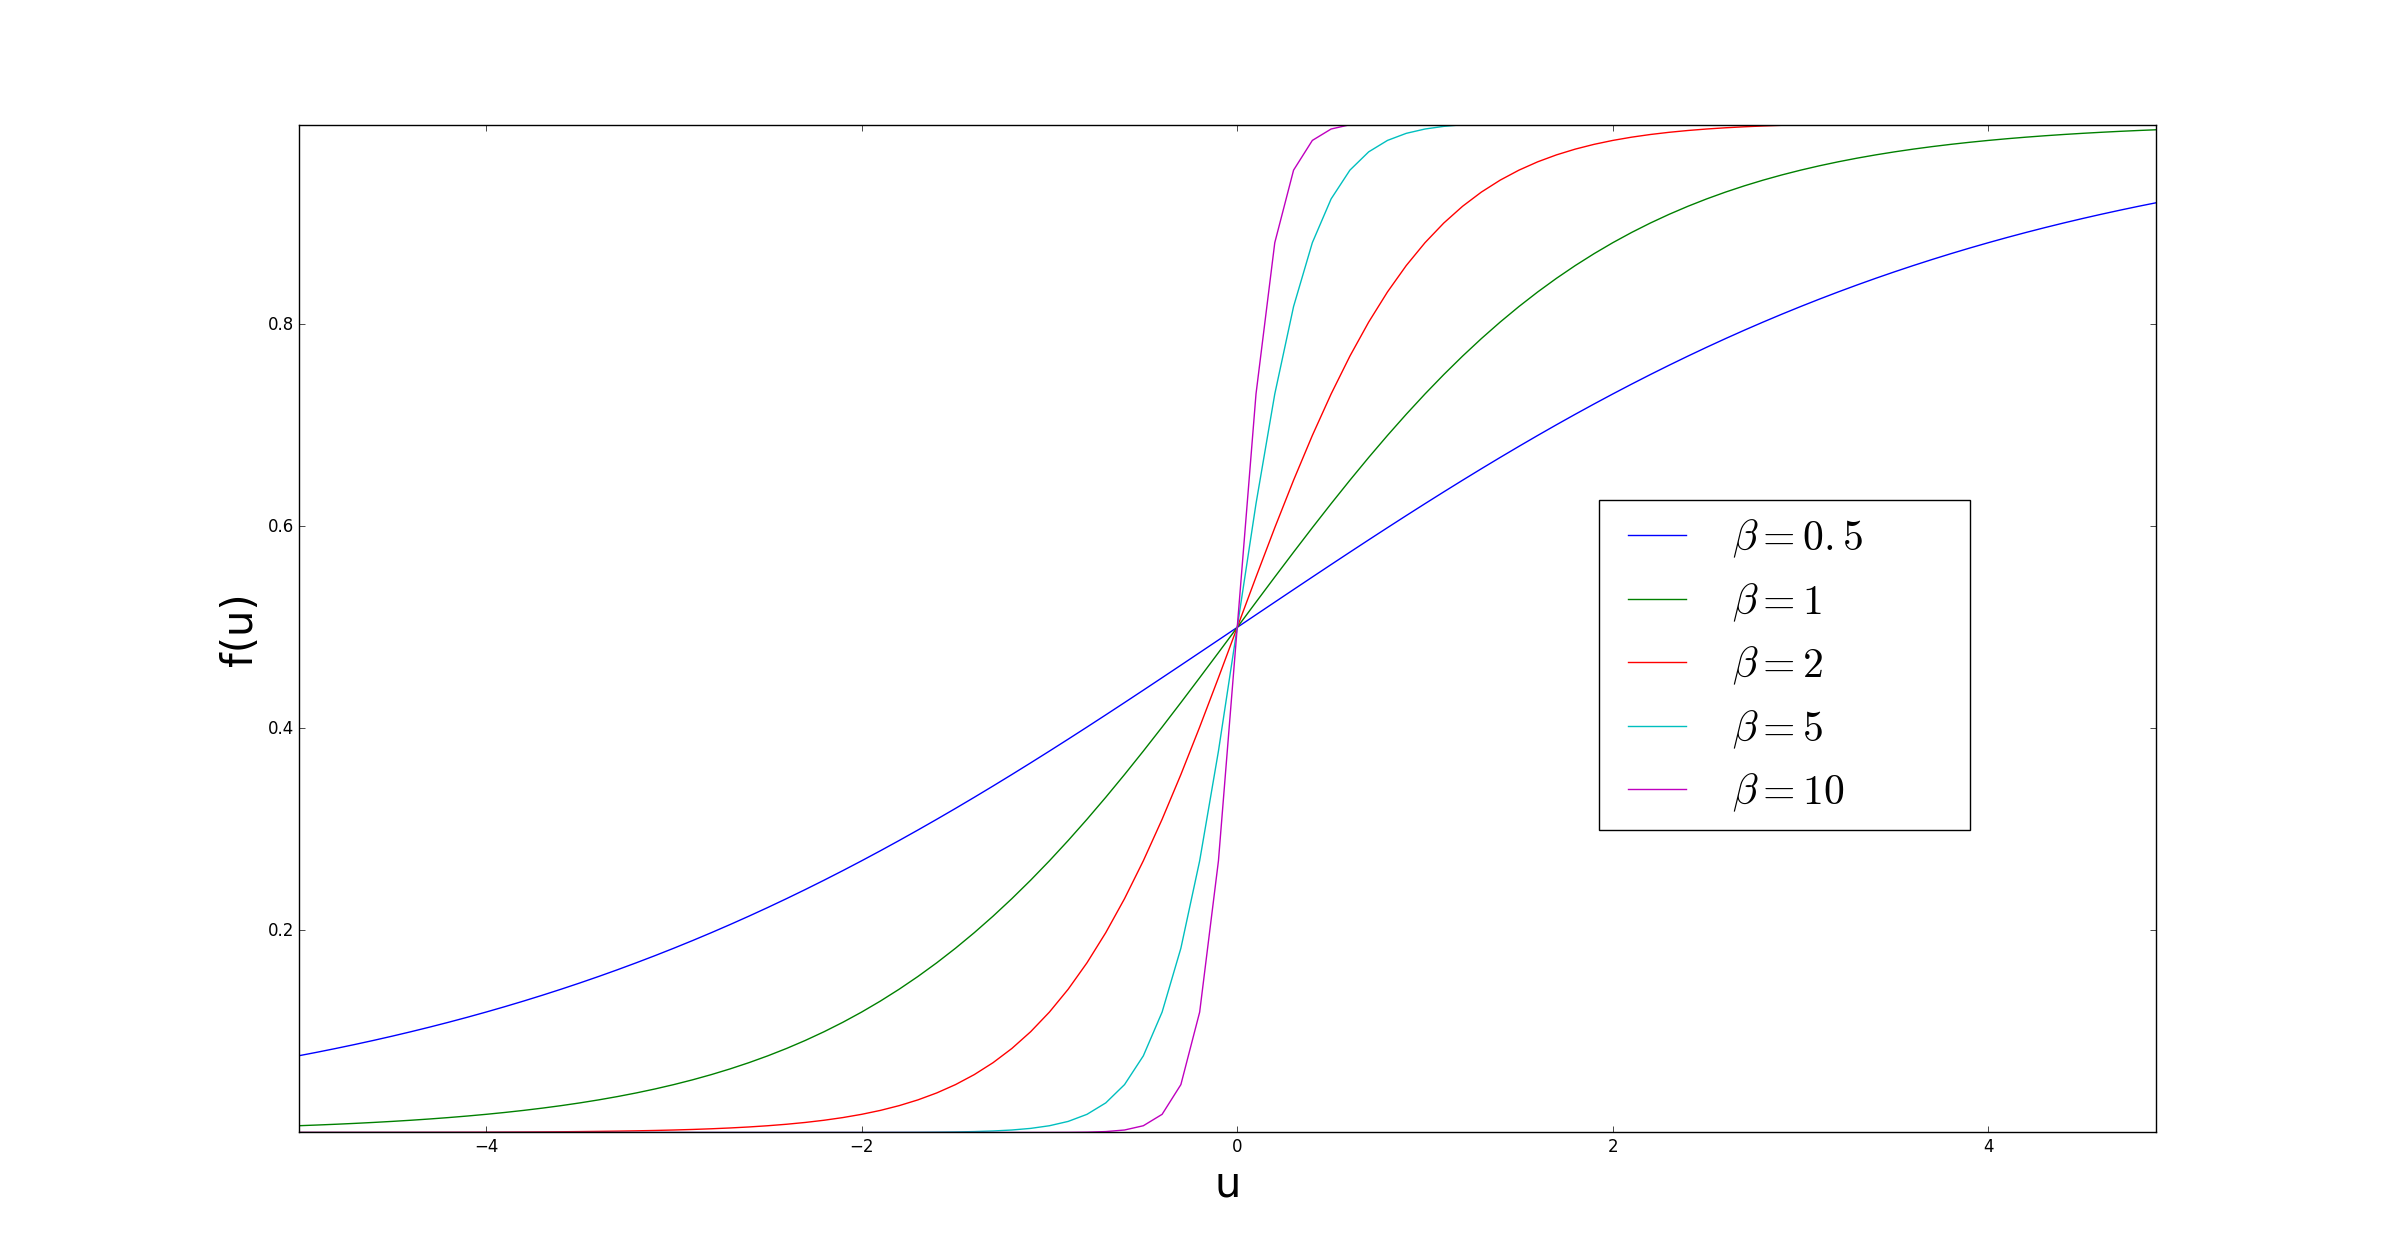
\includegraphics[width=\textwidth]{aktywacja.png}
\caption{Sigmoidalna funkcja unipolarna}
\label{fig:aktywacja}
\end{figure}

Parametr $\beta$ decyduje o kształcie funkcji aktywacji, przy $\beta \rightarrow \infty$ funkcja przechodzi w funkcję skokową. W praktyce zazwyczaj przyjmowana jest wartość $\beta = 1$ \cite{osow01}. Wykres funkcji dla różnych wartości parametru $\beta$ przedstawiono na rysunku \ref{fig:aktywacja}. Istotną właściwością takiej funkcji aktywacji jest jej ciągłość i różniczkowalność, ponieważ pozwala to na skorzystanie z algorytmów gradientowych w procesie uczenia.



\section{Struktura wielowarstwowej sieci perceptronowej}
\label{Sec:ThMLP}
Wielowarstwowa sieć perceptronowa to neurony ułożone w wiele warstw. Wejściami każdego neuronu są wszystkie wyjścia z warstwy poprzedzającej, a jego wyjście jest wejściem dla wszystkich neuronów warstwy następnej. W sieci wielowarstwowej zawsze istnieje jedna warstwa wejściowa, przynajmniej jedna warstwa ukryta i jedna warstwa wyjściowa. Na rysunku \ref{fig:mlp02} przedstawiono sieć wielowarstwową o trzech wejściach w warstwie wejściowej (Input), pięciu neuronach w warstwie ukrytej (Hidden) i dwóch neuronach wyjściowych (Output).

\begin{figure}[H]
\begin{center}
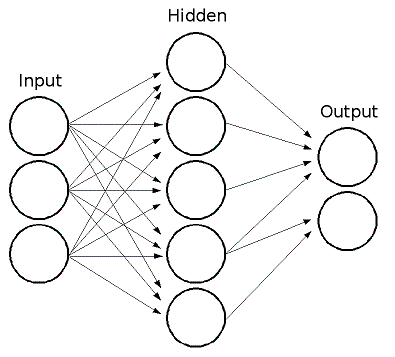
\includegraphics[width=0.5\textwidth]{mlp02.png}
\caption{Wielowarstwowa sieć perceptronowa \\ (źródło: http://docs.opencv.org)}
\label{fig:mlp02}
\end{center}
\end{figure}

Proces uczenia sieci MLP opiera się na prezentacji próbek uczących, porównywaniu odpowiedzi sieci z wartością oczekiwaną, a następnie odpowiedniej korekcji wag połączeń pomiędzy neuronami. Model uczenia, w którym posiadamy oczekiwane odpowiedzi sieci wraz z danymi wejściowymi nazywany jest uczeniem nadzorowanym (ang. supervised learning). 




\section{Propagacja wsteczna}
\label{Sec:ThBackprop}
Algorytm propagacji wstecznej wykorzystuje gradientowe metody optymalizacji w celu dokonywania odpowiednich modyfikacji wag sieci. Jest uważany za jeden ze skuteczniejszych algorytmów uczenia sieci wielowarstwowej \cite{osow01}. Jego wielką zaletą jest wydajność - dzięki odwróceniu kierunku wykonywane jest mnożenie macierzy z wektorami (zamiast macierzy z macierzami), co znacznie zmniejsza koszt obliczeniowy \cite{pml01}. W celu zastosowania algorytmu propagacji wstecznej należy wybrać funkcję kosztu (nazywaną również funkcją celu), której wartość będzie minimalizowana. Często stosowaną funkcją celu jest suma kwadratów różnic między wartościami oczekiwanymi, a wartościami otrzymanymi na wyjściu sieci: $$ E(w)=\frac{1}{2}\sum_{i=1}^{N}(y_i-d_i)^2,$$ gdzie $i$ to numer próbki, $w$ - wagi sieci, $y$ - odpowiedź otrzymana od sieci, a $d$ to oczekiwana odpowiedź. Algorytm propagacji wstecznej działa w kilku krokach. Najpierw następuje obliczenie odpowiedzi sieci na prezentowany wektor wejściowy. Aby uzyskać sygnał wyjściowy sieci, należy podać na jej wejście próbkę uczącą i obliczyć wszystkie wartości pośrednie. Następnym krokiem jest obliczenie aktualnej wartości funkcji kosztu $E(w)$. Kolejno następuje odwrócenie kierunku przepływu w sieci i minimalizacja funkcji celu za pomocą gradientowych metod optymalizacji.


\section{Algorytm najszybszego spadku}
\label{Sec:ThGrad}
Algorytm największego spadku gradientu to jedna z podstawowych i najprostszych gradientowych metod optymalizacji. Ze względu na swoją prostotę posiada wady - jest wolnozbieżny (liniowo), a w miejscach gdzie wartość gradientu jest bardzo mała (okolice punktu optymalnego), postęp jest prawie niezauważalny. Algorytm największego spadku gradientu przez wiele lat był podstawową metodą uczenia wielowarstwowych sieci neuronowych \cite{osow01}, jednak obecnie można już go uznać za algorytm historyczny, używany raczej w celach edukacyjnych.

Istnieją różne wariacje tego algorytmu, które poprawiają jego działanie (zwykle w~sposób heurystyczny). Jedną z takich metod jest metoda nauki z momentem (rozpędem), która oprócz aktualnej wartości gradientu uwzględnia również poprzednią zmianę wag.

\chapter{Przygotowanie danych statystycznych}
Posiadanie odpowiedniej ilości należycie przygotowanych danych to warunek niezbędny do przeprowadzenia procesu uczenia sztucznej sieci neuronowej, a w rezultacie powodzenia całego eksperymentu. Zgromadzenie i odpowiednie przetworzenie danych jest często najbardziej skomplikowaną i najbardziej czasochłonną częścią całego projektu. 

W trakcie poszukiwania i przygotowywania danych można napotkać wiele problemów:
\begin{tightitemize}
\item Brak dostępnych danych lub ich zbyt mała liczba
\item Dane nieaktualne
\item Różne formaty/postacie danych, konieczność ujednolicenia
\item Dane niskiej jakości, wybrakowane lub zniekształcone
\end{tightitemize}

Jakość danych ma znaczny wpływ na jakość wyników analizy, dlatego cały proces przygotowania danych powinien zostać przeprowadzony ze szczególną starannością. Przygotowanie danych może składać się z kilku zadań: wyboru odpowiednich danych, integracji danych pochodzących z różnych źródeł, transformacji danych do pożądanego formatu, odrzucenia nieistotnych/zniekształconych danych. Etap ten jest tak istotny, że w zadaniach analizy danych może zajmować nawet 50-70\% czasu trwania całego projektu \cite{satt01}.

\section{Baza danych}
\label{Sec:DataBase}
Istnieje wiele serwisów internetowych zajmujących się kolekcjonowaniem statystyk tenisa ziemnego. Korzystanie z takich danych nie jest jednak wygodne z perspektywy programisty - serwisy zazwyczaj nie udostępniają publicznego interfejsu, więc pobieranie danych wiązałoby się z wydobywaniem ich bezpośrednio ze stron WWW (ang. \textit{web scraping}). Mogłoby to w wielu przypadkach naruszać również warunki korzystania z tych serwisów.

Poszukując odpowiedniego zbioru danych można trafić na bazy meczów w formacie CSV (ang. \textit{comma-separated values}, wartości rozdzielone przecinkiem). Są one często dystrybuowane na licencjach otwartych, pozwalających na dowolne ich wykorzystywanie. Format CSV jest atrakcyjny dla programisty, bardzo wygodny w użyciu. Niestety dane w~takich bazach bywają wybrakowane lub uszkodzone. Początkowo próbowano wykorzystać jedną z takich baz\footnote{Darmowa baza danych rozpowszechniana na licencji \textit{Creative Commons Attribution-NonCommercial-ShareAlike 4.0 International License}, dostępna pod adresem: \url{https://github.com/JeffSackmann/tennis_atp}}, jednak napotkano pewne problemy. Baza nie była aktualizowana od lutego 2016 roku, a pewne dane były uszkodzone - numery identyfikacyjne graczy niekiedy się powtarzały. Uniemożliwiło to wykorzystanie jej w projekcie.

Kolejną możliwością jest skorzystanie z aplikacji desktopowej. Nie ma ich wiele, większość takich aplikacji nie jest już wspierana. Jednym z ciągle utrzymywanych programów, który wykorzystano w niniejszej pracy jest \textit{OnCourt}. Jego baza danych jest codziennie aktualizowana. Sam program umożliwia przeglądanie wielu statystyk - wszystkie mecze wybranego zawodnika, gry na danej nawierzchni czy w wybranych turniejach, obecna i historyczne pozycje w rankingu, stosunek head-to-head\footnote{Bezpośrednie konfrontacje pomiędzy dwoma wybranymi zawodnikami.} i wiele innych. Baza danych i ilość możliwości jest naprawdę ogromna, jednak wszystko to dostępne jest z poziomu graficznego interfejsu użytkownika, co znacznie utrudnia wygodne korzystanie z tego rozwiązania. Po nawiązaniu kontaktu z firmą KAN-soft, producentem oprogramowania \textit{OnCourt}, otrzymano hasło do lokalnej bazy danych pobieranej przez program, co umożliwiło wysyłanie własnych zapytań do bazy danych. 

\begin{figure}
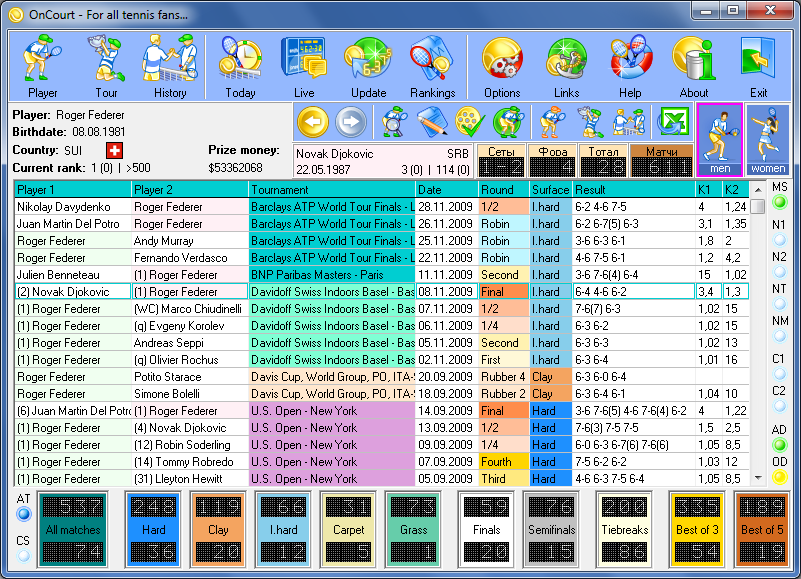
\includegraphics[width=\textwidth]{oncourt1.png}
\caption{Program OnCourt \\ (źródło: http://www.oncourt.info/)}
\label{fig:oncourt1}
\end{figure}

\section{Zastosowane technologie}
\label{Sec:DataTech}
Moduł odpowiadający za pobieranie danych z bazy, a następnie ich przetworzenie został zaimplementowany w języku Python. Python to wysokopoziomowy język skryptowy, który charakteryzuje się rozbudowanym zestawem wbudowanych bibliotek, oraz łatwością instalacji i mnogością modułów zewnętrznych.
Baza danych programu \textit{OnCourt} jest zapisywana z rozszerzeniem \textit{.mdb} - plik bazodanowy programu Microsoft Access. Do połączenia z bazą danych wykorzystano zewnętrzny moduł \textit{pyodbc}. Moduł ten pozwala na połączenie z bazami danych ODBC\footnote{Open DataBase Connectivity - interfejs umożliwiający aplikacjom dostęp do danych w bazie}. Aby było możliwe połączenie z bazą Microsoft Access, należy posiadać zainstalowane sterowniki \textit{Microsoft Access Driver (*.mdb, *.accdb)}, które dostępne są tylko dla systemu operacyjnego Windows. Po odpowiednim podłączeniu do bazy danych można wykonywać dowolne zapytania w języku SQL, a wyniki otrzymywać i przetwarzać w swoim programie. Początkowo napotkano pewne problemy z szybkością działania bazy danych, jednak po założeniu indeksów na odpowiednie pola nastąpiła znacząca poprawa wydajności.

\section{Wykorzystane statystyki}
\label{Sec:DataUsed}
Dane statystyczne wykorzystane do predykcji wyniku muszą odpowiadać danym, którymi dysponowano przed rozegraniem meczu. 
Przykładowo, aby dokonać predykcji zwycięzcy meczu między zawodnikiem A i zawodnikiem B odbywającym się w dniu 25.04.2013, należy pobrać stan z tego dnia przed rozegraniem meczu. W projekcie nie uwzględniono sytuacji, w której zawodnik może rozegrać więcej niż jeden mecz w ciągu jednego dnia, gdyż sytuacja taka ma miejsce niezwykle rzadko (głównie z powodu niesprzyjających warunków atmosferycznych powodujących opóźnienie w rozgrywaniu turnieju). Dane pobierane są na dzień poprzedzający rozegranie meczu. Wszystkie dane zostały znormalizowane i~końcowe wartości używane w procesie przewidywania mają wartość z przedziału $\langle 0, 1\rangle$. 

Poniżej przedstawiono wszystkie dane statystyczne wykorzystane w projekcie, ich oznaczenia używane w dalszej części pracy, oraz krótkie uzasadnienie wyboru i sposób ich uzyskiwania:
\begin{enumerate}
\item R - Ranking zawodnika.

$R = \frac{Ranking\ zawodnika}{900}$

W przypadku braku danych: $R = 1$

Uzasadnienie: ogólna dyspozycja zawodnika w obecnym sezonie.

\item WS - Stosunek wygranych meczów do wszystkich meczów rozegranych przez zawodnika w bieżącym sezonie.

$WS = \frac{Wygrane\ mecze\ zawodnika\ w\ obecnym\ sezonie}{Wszystkie\ mecze\ zawodnika\ w\ obecnym\ sezonie}$

W przypadku braku danych: $WS = 0.4$

Uzasadnienie: ogólna dyspozycja zawodnika w obecnym sezonie.

\item WM - Stosunek wygranych meczów do wszystkich meczów rozegranych przez zawodnika w ciągu ostatnich dwóch miesięcy.

$WM = \frac{Wygrane\ mecze\ zawodnika\ ostatnie\ 2\ mies.}{Wszystkie\ mecze\ zawodnika\ ostatnie\ 2\ mies.}$

W przypadku braku danych: $WM = 0.4$

Uzasadnienie: dyspozycja zawodnika w ciągu ostatnich dwóch miesięcy.

\item WC - Stosunek wygranych meczów do wszystkich meczów rozegranych przez zawodnika na korcie danego typu.

$WC = \frac{Wygrane\ mecze\ zawodnika\ na\ kortach\ danego\ typu}{Wszystkie\ mecze\ zawodnika\ na\ kortach\ danego\ typu}$

W przypadku braku danych: $WC = 0.4$

Uzasadnienie: rodzaj nawierzchni, na której rozgrywany będzie mecz ma ogromne znaczenie w tenisie. Niektórzy zawodnicy radzą sobie zdecydowanie lepiej na jednej z nawierzchni. Przykładem może być Stanislas Wawrinka, który na dzień 29.11.2016 na kortach ziemnych wygrał 69\% spośród 356 meczów, podczas gdy na kortach trawiastych jest to 54\% z jedynie 50 meczów.

\item WT - Stosunek wygranych meczów do wszystkich meczów rozegranych przez zawodnika w danym turnieju. Brane są pod uwagę wszystkie dotychczasowe edycje turnieju, w których zawodnik brał udział.

$WT = \frac{Wygrane\ mecze\ zawodnika\ w\ danym\ turnieju}{Wygrane\ mecze\ zawodnika\ w\ danym\ turnieju}$

W przypadku braku danych: $WT = 0.4$

Uzasadnienie: zdarza się, że zawodnik notuje wyjątkowo dobre lub wyjątkowo słabe występy w konkretnym turnieju.

\item GD - Łączna liczba gemów rozegranych przez zawodnika w ciągu ostatnich 3 dni.

$GD = N,$ gdzie $N$ to łączna liczba gemów rozegranych przez zawodnika w ciągu 3~dni poprzedzających przewidywany mecz.

Uzasadnienie: duża liczba gemów rozegranych przez zawodnika w dniach poprzedzających mecz może decydować o jego zmęczeniu.

\item H2H - Stosunek head-to-head między dwoma zawodnikami.

$H2H = \frac{Wygrane\ mecze\ zawodnika\ w\ starciu\ z\ danym\ przeciwnikiem}{Wszystkie\ mecze\ zawodnika\ w\ starciu\ z\ danym\ przeciwnikiem}$

W przypadku braku danych: $H2H = 0.5$

H2H obliczane jest tylko dla jednego z graczy występujących w meczu. Stosunek H2H dla drugiego z graczy (H2HB) w oczywisty sposób wynika z wartości H2H i~wynosi $H2HB = 1 - H2H$. Z tego powodu parametr H2HB nie jest wykorzystywany.

Uzasadnienie: czasami styl gry jednego zawodnika nie odpowiada innemu zawodnikowi i jeden z nich wygrywa zdecydowaną większość spotkań.

\end{enumerate}

\section{Zwiększenie ilości danych}
\label{Sec:DataDouble}

W celu zwiększenia ilości posiadanych danych, oraz zmniejszenia wrażliwości sieci na kolejność podawania zawodników biorących udział w meczu, statystyki wszystkich meczów zostały zdublowane z zamienioną kolejnością zawodników. Poniżej przedstawiono przykład postępowania dla jednego meczu:

Rozegrany został mecz między zawodnikiem A i zawodnikiem B. Zawodnik A wygrał. Wektor danych wejściowych mógłby wyglądać następująco\footnote{Wektor celowo został przedstawiony w trzech liniach, aby oddzielić statystyki gracza A od gracza B.}: $$[R_A, WS_A, WM_A, WC_A, WT_A, GD_A,$$
$$H2H_A,$$  
$$R_B, WS_B, WM_B, WC_B, WT_B, GD_B]$$
Odpowiadający mu wektor wyjściowy: $$[1, 0]$$

Dla podanego przykładu wygenerowano odpowiadające mu wektory wejścia i wyjścia z zamienioną kolejnością zawodników:
$$[R_B, WS_B, WM_B, WC_B, WT_B, GD_B,$$
$$1-H2H_A,$$  
$$R_A, WS_A, WM_A, WC_A, WT_A, GD_A]$$
Odpowiadający wektor wyjściowy: $$[0, 1]$$

W wyniku tego działania całkowita ilość danych zwiększyła się dwukrotnie.

\chapter{Implementacja sieci neuronowej}
\section{Uniwersalny moduł MLP}
\label{Sec:MLPMod}

Celem było zaimplementowanie uniwersalnego modułu MLP (MultiLayer Perceptron - perceptron wielowarstwowy), którego będzie można dowolnie dostosowywać w zależności od potrzeb. Dotyczy to w szczególności architektury sieci (ilości wejść, ilości neuronów w warstwach ukrytych, ilości neuronów wyjściowych) oraz wykorzystywanych funkcji aktywacji, funkcji kosztów czy hiperparametrów (współczynnik uczenia, współczynnik momentu).

\section{Zastosowane technologie}
\label{Sec:MLPTech}
Moduł MLP zaimplementowano wykorzystując język Python. Do wykonywania obliczeń macierzowych użyto zewnętrznej biblioteki NumPy. NumPy to pakiet wykorzystywany do wykonywania obliczeń naukowych, a w szczególności do szybkiego przetwarzania \\ N-wymiarowych tablic. Umożliwia wykonywanie obliczeń specyficznych dla macierzy oraz łatwe wykonywanie działań element po elemencie.


\section{Struktura programu}
\label{Sec:MLPStruct}
Moduł MLP składa się z jednej klasy reprezentującej całą sieć neuronową - MLP. Zdecydowano o takiej konstrukcji, ponieważ wagi sieci przechowywane są w tablicach numpy.ndarray. Przejście sygnału przez sieć sprowadza się do wykonywania odpowiednich działań na macierzach. Utworzenie oddzielnej klasy odpowiadającej za Neuron i stworzenie sieci z obiektów klasy Neuron, skutkowałoby koniecznością wywoływania odpowiednich funkcji klasy Neuron dla każdego obiektu. Znacznie spowolniłoby to działanie całego programu. Diagram UML klasy MLP przedstawiono na rysunku \ref{fig:mlp01}.

\begin{figure}
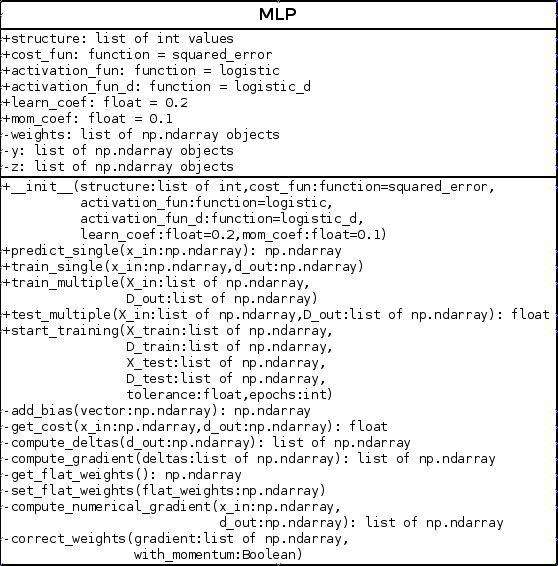
\includegraphics[width=\textwidth]{mlp01.png}
\caption{Diagram UML klasy MLP}
\label{fig:mlp01}
\end{figure}

\pagebreak

\section{Interfejs programisty}
\label{Sec:MLPAPI}

Aby skorzystać z klasy MLP wystarczy znajomość jedynie kilku metod. Proces korzystania z modułu MLP można podzielić na trzy etapy:
\begin{enumerate}
\item Stworzenie sieci o wybranej architekturze

Do stworzenia sieci o wybranej architekturze należy wykorzystać konstruktor klasy MLP. Jedynym niezbędnym parametrem jest pożądana struktura sieci, podawana w formie listy całkowitych liczb dodatnich, np. $[2, 3, 1]$ - sieć o dwóch wejściach, 3 neuronach w warstwie ukrytej i jednym neuronie wyjściowym. Pozostałe, opcjonalne parametry wraz z wartościami domyślnymi:

\begin{tightitemize}
\item cost\_fun (funkcja) - funkcja kosztu służąca do obliczenia wartości błędu. Domyślnie jest to błąd kwadratowy przemnożony przez 0.5.
\item activation\_fun (funkcja) - funkcja aktywacji. Domyślnie funkcja logistyczna - sigmoidalna funkcja unipolarna.
\item activation\_fun\_d (funkcja) - pochodna funkcji aktywacji. Domyślnie pochodna unipolarnej funkcji sigmoidalnej.
\item learn\_coef (float) - współczynnik uczenia. Wartość domyślna: 0.2.
\item mom\_coef (float) - współczynnik momentu. Wartość domyślna: 0.1
\end{tightitemize}

\item Przeprowadzenie procesu uczenia

Gdy obiekt klasy MLP jest już stworzony, można rozpocząć proces uczenia sieci. Ogranicza się to do wywołania metody start\_training. Niezbędnymi parametrami są zbiory danych: X\_train (wejściowe dane uczące), Y\_train (pożądane wyjścia odpowiadające danym podanym jako argument X\_train), X\_test (wejściowe dane testowe), Y\_test (pożądane wyjścia odpowiadające danym podanym jako argument X\_train). Opcjonalne parametry to epochs (maksymalna liczba epok\footnote{Epoka w procesie uczenia sieci neuronowych to przetworzenie całego ciągu danych uczących.}) i tolerance (gdy średni błąd spadnie poniżej tej wartości nastąpi zakończenie procesu uczenia). Zastosowano typ uczenia on-line\footnote{Typ uczenia on-line: Wagi sieci uaktualniane są po każdym przetworzonym przykładzie wejściowym. }.

\item Wykorzystywanie nauczonej sieci
W celu otrzymania odpowiedzi sieci na wektor danych wejściowych należy trzeba posłużyć się metodą predict\_single, jako argument podając jeden wektor danych wejściowych. Zwrócony zostanie wektor wyjściowy wygenerowany przez sieć.
\end{enumerate}

\pagebreak

Przykładowe zastosowanie modułu MLP do rozwiązania problemu XOR:
\begin{verbatim}
# Inicjalizacja danych wejściowych i wyjściowych
in = np.array(([1, 1], [1, 0], [0, 1], [0, 0]), dtype=float)
out = np.array(([0], [1], [1], [0]), dtype=float)

# Utworzenie sieci o strukturze: 2 wejścia, 3 neurony w warstwie 
# ukrytej, 1 neuron wyjściowy. Pozostałe parametry domyślne.
net = MLP([2, 3, 1])

# Rozpoczęcie treningu dla danych problemu XOR. Dane treningowe 
# identyczne jak dane testowe. Liczba epok 10000, gdy wartość
# błędu spadnie poniżej 0.001, nastąpi zakończenie procesu uczenia.
net.start_training(in, out, in, out, epochs=10000, tolerance=0.001)

# Wykorzystanie nauczonej sieci do predykcji
for x in in:
    net.predict_single(x)
\end{verbatim}



\chapter{Przeprowadzone doświadczenia}

Wszystkie doświadczenia przeprowadzono na komputerze o procesorze Intel Core i3-3110M 2.40 GHz i 4 GB pamięci RAM. W wynikach eksperymentów przedstawiono uzyskane wyniki przewidywania wraz z czasami trwania procesu uczenia dla różnych wariantów sieci i różnych wektorów uczących.

Wykorzystane w procesie uczenia mecze pochodzą z największych turniejów tenisowych z lat 2002-2016. Dane treningowe i dane testowe składają się ze 150 tysięcy losowo wybranych i niepowtarzających się meczów.

\section{Porównanie wyników dla różnych wektorów danych wejściowych}
\label{Sec:VsXIn}

Pierwszym przeprowadzonym eksperymentem było podawanie różnych danych statystycznych na wejście sieci o stałej strukturze. Do tego doświadczenia wybrano model o jednej warstwie ukrytej składającej się z 10 neuronów - $H_{10}$. 

Wektory danych wejściowych podawanych na wejście sieci:
\begin{tightitemize}
\item $X_4$: Dane bardzo ogólne, 3 parametry - ranking zawodników, procent wygranych meczów w obecnym sezonie:
$$[R_A, WS_A, R_B, WS_B]$$
\item $X_{8A}$: $X_{4}$ rozszerzone o procent wygranych w ciągu ostatnich dwóch miesięcy i powodzenie gracza na danym rodzaju nawierzchni:
$$[R_A, WS_A, WM_A, WC_A, R_B, WS_B, WM_B, WC_B]$$
\item $X_{8B}$: Dane podobne jak $X_{8A}$, jedyną różnicą jest podawanie sukcesu gracza w danym turnieju zamiast rodzaju nawierzchni:
$$[R_A, WS_A, WM_A, WT_A, R_B, WS_B, WM_B, WT_B]$$
\item $X_{13}$: Wektor zawierający wszystkie 13 parametrów:
$$[R_A, WS_A, WM_A, WC_A, WT_A, GD_A,H2H_A,R_B, WS_B, WM_B, WC_B, WT_B, GD_B]$$
\end{tightitemize}

Proces uczenia przeprowadzono ze współczynnikiem uczenia wynoszącym 0.2 oraz współczynnikiem momentu równym 0.1. Ustalono ilość epok równą 15. Wyniki procesu uczenia przedstawiono w tabeli \ref{tab:xacc}.

\begin{table}
\centering
\caption{Skuteczność sieci $H_{10}$ dla różnych wektorów wejściowych}
\label{tab:xacc}
\begin{tabular}{|l|l|l|l|l|}
\hline
\textbf{Epoka} & \textbf{$X_4$} & \textbf{$X_{8A}$} & \textbf{$X_{8B}$} & \textbf{$X_{13}$} \\ \hline
1              & 66.93\%     & 70.43\%      & 77.90\%      & 84.49\%      \\ \hline
2              & 67.21\%     & 70.65\%      & 77.92\%      & 84.80\%      \\ \hline
3              & 67.50\%     & 70.81\%      & 77.93\%      & 85.07\%      \\ \hline
4              & 67.62\%     & 70.93\%      & 77.94\%      & 85.17\%      \\ \hline
5              & 67.66\%     & 70.99\%      & 77.96\%      & 85.38\%      \\ \hline
6              & 67.67\%     & 71.04\%      & 77.98\%      & 85.58\%      \\ \hline
7              & 67.72\%     & 71.07\%      & 77.98\%      & 85.71\%      \\ \hline
8              & 67.72\%     & 71.11\%      & 78.03\%      & 85.77\%      \\ \hline
9              & 67.73\%     & 71.15\%      & 78.08\%      & 85.83\%      \\ \hline
10             & 67.74\%     & 71.18\%      & 78.16\%      & 85.89\%      \\ \hline
11             & 67.76\%     & 71.20\%      & 78.23\%      & 85.93\%      \\ \hline
12             & 67.77\%     & 71.21\%      & 78.29\%      & 85.99\%      \\ \hline
13             & 67.77\%     & 71.20\%      & 78.34\%      & 86.03\%      \\ \hline
14             & 67.77\%     & 71.18\%      & 78.35\%      & 86.05\%      \\ \hline
15             & 67.79\%     & 71.18\%      & 78.35\%      & 86.06\%      \\ \hline
\end{tabular}
\end{table}

Ilość danych uczących wynosząca 150 tysięcy oraz zastosowanie uczenia w trybie online powoduje, że już po pierwszej epoce sieć uzyskuje bardzo dobre wyniki. W~kolejnych epokach skuteczność zmienia się nieznacznie. Spowodowane jest to małymi zmianami wagi sieci wynikającymi z niskich wartości obliczanego gradientu. Sugeruje to, że wartości funkcji kosztu dla takich wag sieci znajdują się w okolicy minimum. Zastosowanie bardziej zaawansowanego algorytmu uczenia sieci najprawdopodobniej wpłynęłoby korzystnie na uzyskiwane rezultaty.

W procesie uczenia zjawisko przeuczenia\footnote{Przeuczenie sieci (ang. overfitting) - zjawisko, w którym sieć za bardzo dopasowuje się do danych uczących, traci zdolność generalizacji. Można je zauważyć, gdy błąd dla zbioru uczącego maleje, jednak na zbiorze testowym błąd zaczyna wzrastać.} sieci wystąpiło jedynie dla przypadku $X_{8A}$ i było minimalne - spadek skuteczności dla zbioru testowego z $71.21\%$ w epoce 12 do $71.18\%$ w epoce 15. Taka sytuacja wynika prawdopodobnie ze specyfiki badanego problemu. Przy tak dużej ilości danych zbiór testowy jest zapewne dość zbliżony do zbioru uczącego.

Dla wektorów wejściowych $X_4$, zawierających jedynie 4 parametry osiągnięto skuteczność prawie 68\%, co jest raczej dobrym wynikiem jak na tak małą ilość parametrów. Ciekawe rezultaty uzyskano dla wektorów $X_{8A}$ i $X_{8B}$, gdzie skuteczność wyniosła odpowiednio 71.18\% i 78.35\%. Ponad 7\% różnicy w osiągniętej skuteczności to bardzo dużo, szczególnie biorąc pod uwagę fakt, że różniły się tylko jedną cechą dla każdego z graczy. Taki rezultat sugeruje, że większe znaczenie ma powodzenie gracza w danym turnieju niż na danej nawierzchni. Przyczyną może być fakt, że dany cykl turnieju odbywa się na jednej konkretnej nawierzchni, zatem informacja o sukcesach w turnieju zawiera w sobie pośrednio część informacji o powodzeniu na tej nawierzchni.

Zdecydowanie największą skuteczność uzyskano wykorzystując wektor $X_{13}$, zawierający wszystkie 13 parametrów. Wynik 86\% jest zaskakująco wysoki, nie oczekiwano osiągnięcia aż tak dobrego rezultatu.

\begin{figure}
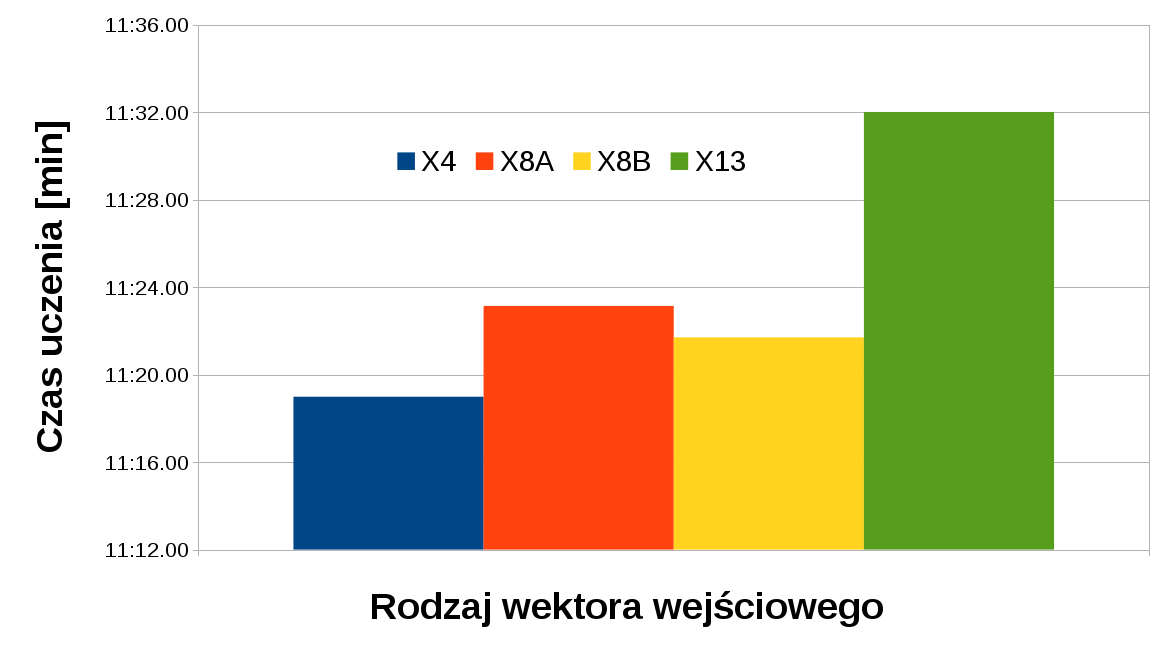
\includegraphics[width=\textwidth]{time_x.png}
\caption{Czas uczenia sieci dla różnych wektorów wejściowych}
\label{fig:timex}
\end{figure}

Pomiar czasu procesu uczenia przyniósł oczekiwane rezultaty. Czas uczenia rośnie wraz ze wzrostem rozmiaru wektorów wejściowych, ponieważ wykonywane jest wtedy więcej operacji. Wzrost czasu uczenia jest jednak nieznaczny, gdyż różnica pomiędzy wektorem wejść o długości 13, a wektorem długości 4 wynosi jedynie 13 sekund, co stanowi niecałe 2\% czasu uczenia wektora $X_4$, podczas gdy wzrost liczby parametrów to 225\%. 

\section{Porównanie wyników dla różnych architektur sieci}
\label{Sec:VsArch}
Dla wektora danych wejściowych $X_{13}$, który uzyskał najlepsze rezultaty w poprzednim podrozdziale, przeprowadzono procesy uczenia dla różnych architektur sieci. 

Wybrane struktury sieci (w nawiasach podano stosowane oznaczenia):
\begin{tightitemize}
\item 1 warstwa ukryta, 1 neuron ($H_{1}$)
\item 1 warstwa ukryta, 3 neurony ($H_{3}$)
\item 1 warstwa ukryta, 10 neuronów ($H_{10}$)
\item 1 warstwa ukryta, 20 neuronów ($H_{20}$)
\item 1 warstwa ukryta, 100 neuronów ($H_{100}$)
\item 2 warstwy ukryte, odpowiednio 10 i 10 neuronów ($H_{10}H_{10}$)
\item 2 warstwy ukryte, odpowiednio 100 i 100 neuronów ($H_{100}H_{100}$)
\end{tightitemize}

Proces uczenia przeprowadzono ze współczynnikiem uczenia wynoszącym 0.2 oraz współczynnikiem momentu równym 0.1. Ustalono ilość epok równą 15. Poniżej przedstawiono tabelę przedstawiającą skuteczności na zbiorze uczącym po każdej epoce wszystkich modeli sieci:

\begin{table}[H]
\centering
\caption{Skuteczność sieci o różnych strukturach na zbiorze testowym}
\label{tab:hacc}
\begin{tabular}{|l|l|l|l|l|l|l|l|}
\hline
\textbf{Epoka} & \textbf{$H_{1}$} & \textbf{$H_{3}$} & \textbf{$H_{10}$} & \textbf{$H_{20}$} & \textbf{$H_{100}$} & \textbf{$H_{10}H_{10}$} & \textbf{$H_{100}H_{100}$} \\ \hline
1              & 82.97\%          & 84.87\%          & 84.38\%           & 84.79\%           & 50.02\%            & 84.01\%                 & 50.02\%                   \\ \hline
2              & 82.97\%          & 85.06\%          & 85.10\%           & 85.31\%           & 50.02\%            & 85.00\%                 & 50.02\%                   \\ \hline
3              & 82.97\%          & 84.99\%          & 85.36\%           & 85.55\%           & 50.02\%            & 85.34\%                 & 50.02\%                   \\ \hline
4              & 82.97\%          & 85.04\%          & 85.52\%           & 85.66\%           & 50.02\%            & 85.47\%                 & 50.02\%                   \\ \hline
5              & 82.97\%          & 85.27\%          & 85.68\%           & 85.74\%           & 50.02\%            & 85.45\%                 & 50.02\%                   \\ \hline
6              & 82.97\%          & 85.33\%          & 85.81\%           & 85.83\%           & 50.02\%            & 85.60\%                 & 50.02\%                   \\ \hline
7              & 82.97\%          & 85.39\%          & 85.89\%           & 85.89\%           & 50.02\%            & 85.78\%                 & 50.02\%                   \\ \hline
8              & 82.97\%          & 85.43\%          & 85.96\%           & 85.98\%           & 50.02\%            & 85.90\%                 & 50.02\%                   \\ \hline
9              & 82.97\%          & 85.44\%          & 86.00\%           & 86.05\%           & 50.02\%            & 85.99\%                 & 50.02\%                   \\ \hline
10             & 82.97\%          & 85.47\%          & 86.04\%           & 86.11\%           & 50.02\%            & 86.07\%                 & 50.02\%                   \\ \hline
11             & 82.97\%          & 85.49\%          & 86.10\%           & 86.17\%           & 50.02\%            & 86.10\%                 & 50.02\%                   \\ \hline
12             & 82.97\%          & 85.50\%          & 86.12\%           & 86.22\%           & 50.02\%            & 86.13\%                 & 50.02\%                   \\ \hline
13             & 82.97\%          & 85.51\%          & 86.16\%           & 86.28\%           & 50.02\%            & 86.20\%                 & 50.02\%                   \\ \hline
14             & 82.97\%          & 85.51\%          & 86.23\%           & 86.28\%           & 50.02\%            & 86.25\%                 & 50.02\%                   \\ \hline
15             & 82.97\%          & 85.52\%          & 86.27\%           & 86.28\%           & 50.02\%            & 86.29\%                 & 50.02\%                   \\ \hline
\end{tabular}
\end{table}

Modele sieci $H_{100}$ i $H_{100}H_{100}$, które miały bardzo dużą ilość neuronów w warstwie ukrytej nie poprawiły swoich rezultatów. Zauważono, że obliczane wartości gradientu były znikome i w żaden sposób nie wpływały na zmianę wag sieci. Pozostałe struktury uzyskały bardzo zadowalające rezultaty przekraczające 82\% poprawnych predykcji. Modele $H_1$ i~$H_3$ posiadające zbyt małą liczbę neuronów osiągnęły nieco niższą, chociaż i tak zaskakująco wysoką skuteczność.

\begin{figure}
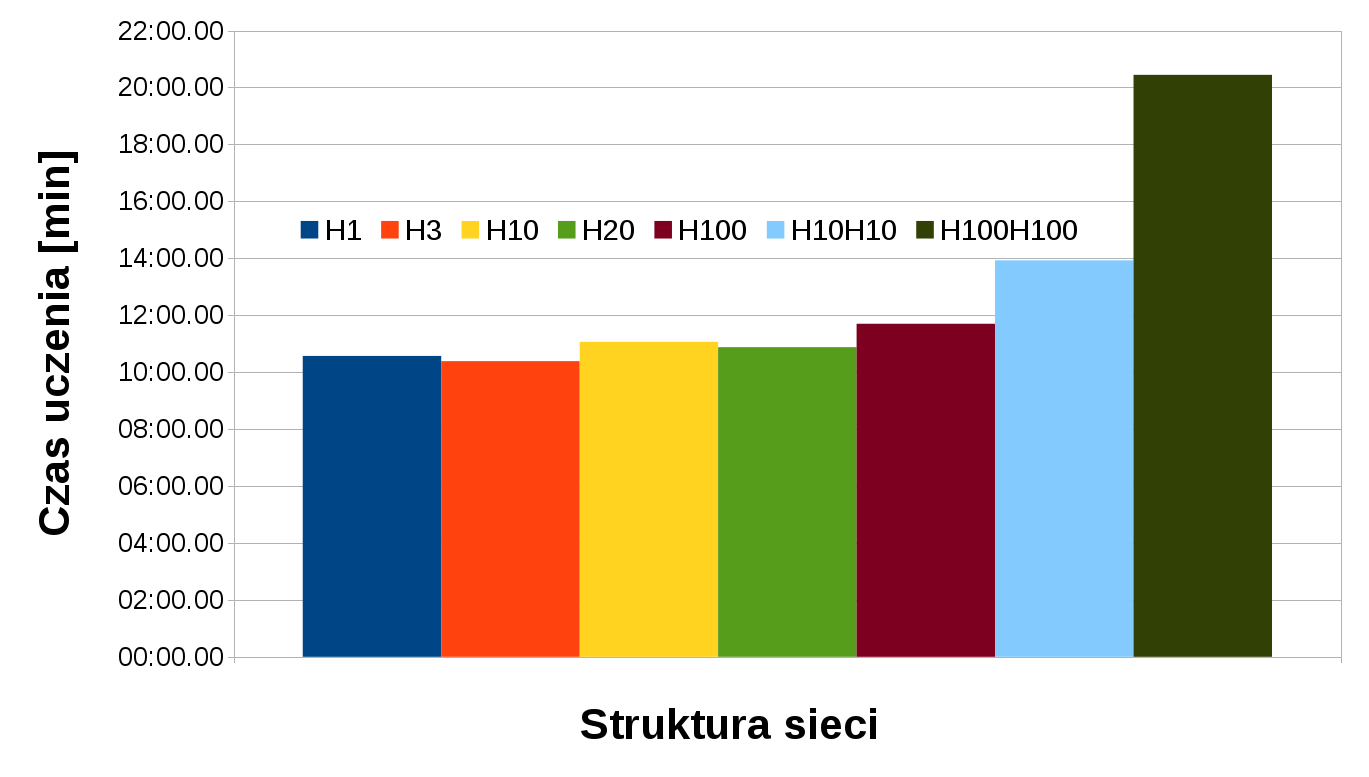
\includegraphics[width=\textwidth]{time_h.png}
\caption{Czas uczenia sieci o różnych ilościach neuronów}
\label{fig:timeh}
\end{figure}

Czas uczenia sieci rośnie wraz ze wzrostem jej struktury (Rys. \ref{fig:timeh}). Jest to szczególnie widoczne przy rozbudowywaniu sieci o kolejne warstwy ukryte, gdzie czas przeprowadzonego procesu uczenia wzrósł o około $30\%$ dla sieci $H_{10}H_{10}$ i prawie dwukrotnie dla $H_{100}H_{100}$. Taka obserwacja była oczekiwana, gdyż wraz ze wzrostem rozmiaru sieci wzrasta liczba wykonywanych operacji. Przeprowadzenie badania dla stałej ilości epok zostało wykonane w celu doświadczalnym. W realnej aplikacji zastosowanie innego warunku stopu dałoby inne rezultaty.

\section{Porównanie z innymi strategiami}
\label{Sec:VsStrat}
Wyniki modelu o 10 neuronach w warstwie ukrytej i 13 parametrach wektora wejściowego porównano z wynikami innych, prymitywnych strategii. Porównywane strategie:
\begin{tightitemize}
\item Losowo - losowy wybór zwycięzcy
\item Ranking - wybór zawodnika plasującego się wyżej w rankingu (losowo w przypadku, gdy żaden z zawodników nie jest sklasyfikowany)
\item H2H - wybór zawodnika o lepszym bilansie head-to-head (losowo w przypadku, gdy zawodnicy nie rozgrywali między sobą żadnego meczu)
\item MLP - wektor danych wejściowych $X_{13}$, architektura sieci $H_{10}$
\end{tightitemize}

\begin{table}[H]
\centering
\caption{Skuteczność różnych strategii wyboru zwycięzcy}
\label{tab:scores}
\begin{tabular}{|l|l|l|l|}
\hline
\textbf{Losowo} & \textbf{Ranking} & \textbf{H2H} & \textbf{MLP} \\ \hline
49.99\%          & 65.92\%            & 63.54\%        & 86.06\%        \\ \hline
\end{tabular}
\end{table}

W tabeli \ref{tab:scores} przedstawiono otrzymane rezultaty dla wszystkich badanych strategii. Wykorzystując model MLP uzyskano zdecydowanie lepsze rezultaty niż losowe, czy bazujące jedynie na jednym parametrze.

\begin{figure}[H]
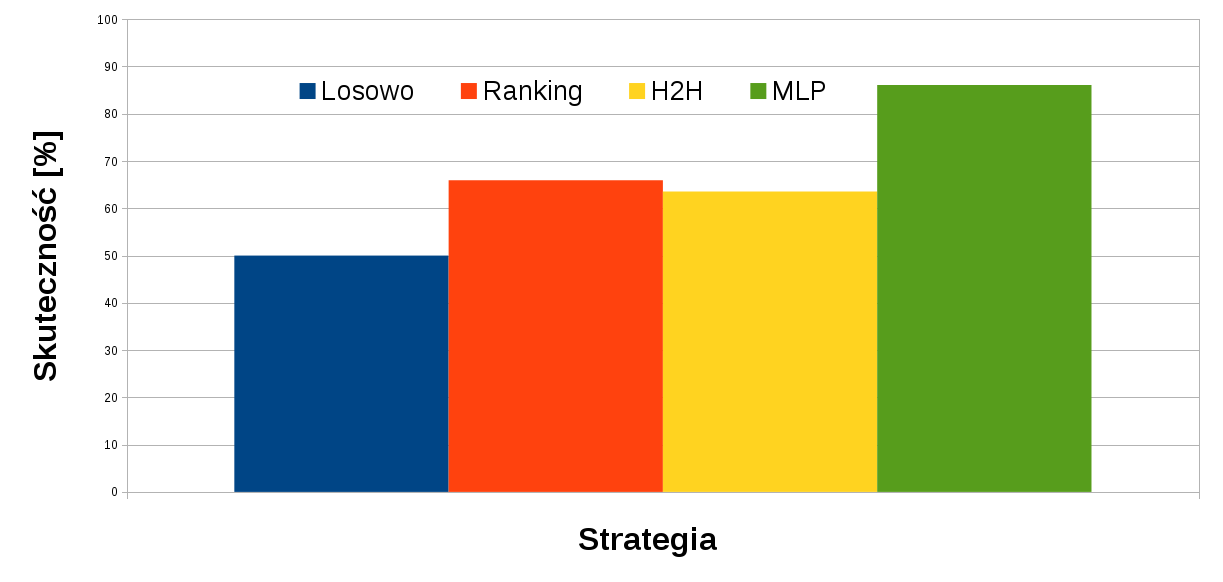
\includegraphics[width=\textwidth]{scores.png}
\caption{Skuteczność różnych strategii wyboru zwycięzcy}
\label{fig:scores}
\end{figure}



\chapter{Publikacja przewidywań na portalu społecznościowym}

\section{Zastosowane technologie}
\label{Sec:BotTech}

Do zaimplementowania programu publikującego przewidywania sieci użyto języka Python oraz biblioteki \textit{twitter}. W celu podłączenia się do profilu na portalu Twitter poprzez bibliotekę \textit{twitter} należy wygenerować i wykorzystać odpowiednie klucze uwierzytelniające. Pozwalają one na identyfikację unikalnego użytkownika, na którego koncie publikowane będą wiadomości.

\section{Predykcje przedmeczowe}
\label{Sec:PredykcjePrzed}
Na portalu Twitter publikowane są przewidywania zwycięzcy w nadchodzących meczach w danym dniu. Przykładowe predykcje zaprezentowano na rysunku \ref{fig:preds}. Informacje o nadchodzących meczach pobierane są bezpośrednio z bazy danych programu OnCourt. Raz dziennie wykonywany jest cykl składający się z trzech etapów:
\begin{tightitemize}
\item Aktualizacja bazy danych
\item Pobranie informacji o nadchodzących meczach
\item Predykcje wyników i ich publikacja
\end{tightitemize}

\begin{figure}
\centering
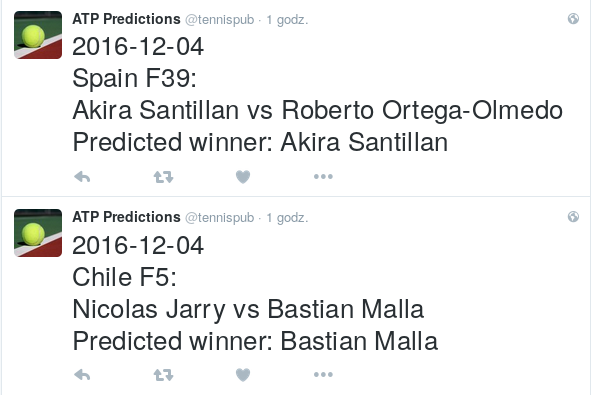
\includegraphics[width=0.5\textwidth]{atp_pred.png}
\caption{Predykcje na portalu Twitter}
\label{fig:preds}
\end{figure}

\chapter{Podsumowanie}
Zgodnie z założonym celem stworzono model sieci neuronowej przewidujący zwycięzcę meczu tenisa ziemnego. Uzyskany rezultat 86\% skuteczności predykcji dla zbioru testowego jest satysfakcjonującym wynikiem. Posiadanie dużej ilości danych wysokiej jakości pozwoliło na zastosowanie uczenia maszynowego do rozwiązania badanego problemu z~dobrym efektem. Predykcje wyników nadchodzących meczów publikowane są na portalu społecznościowym Twitter.

Istnieje wiele zewnętrznych bibliotek pozwalających na szybkie i łatwe korzystanie z~gotowych modeli sieci neuronowych (np. PyBrain, Keras). Wykorzystywanie takich bibliotek to obecnie najpopularniejsze podejście - pozwala skupić się na rozwiązywanym problemie, kolekcjonowaniu i przygotowywaniu danych, a pominąć etap implementowania modelu. Zdecydowano jednak stworzyć moduł MLP samodzielnie w celu lepszego poznania zasad działania sieci neuronowych. Pozwoliło to zauważyć pojawiające się problemy. Moduł MLP zaimplementowano w sposób pozwalający na łatwe dostosowanie go do innych zadań. Wymagany jest jedynie dobór odpowiedniej struktury sieci oraz posiadanie stosownych zbiorów danych. Zastosowanie algorytmu najszybszego spadku gradientu dało całkiem niezłe rezultaty, jednak znanych jest wiele algorytmów które działają znacznie efektywniej. Ważnym etapem w procesie uczenia sieci była standaryzacja danych. Przed ustandaryzowaniem danych efekty działania algorytmu najszybszego spadku gradientu były bardzo słabe - postęp w procesie uczenia był niemal niezauważalny. 

Największe trudności napotkano na etapie przygotowywania danych. Przed znalezieniem programu \textit{OnCourt} próbowano korzystać z innych źródeł, jednak we wszystkich przypadkach napotykano problemy związane najczęściej z niekompletnością i nieaktualnością bazy. Przetwarzanie stron WWW w celu zdobycia potrzebnych danych byłoby trudnym zadaniem i wymagałoby wielkiego nakładu pracy. Skorzystanie z bazy danych programu \textit{OnCourt} znacznie ułatwiło rozwój projektu.

Przeprowadzone doświadczenia wykazały, że stworzony model radzi sobie zdecydowanie lepiej niż prymitywne strategie bazujące na pojedynczych parametrach. W wykonanych badaniach najlepsze rezultaty zostały uzyskane dla wektora zawierającego największą liczbę danych statystycznych. Wszystkie wykorzystane dane zdają się być istotne w~procesie przewidywania zwycięzcy. Dobór ilości neuronów w warstwach ukrytych odbywa się zazwyczaj eksperymentalnie. Aby osiągnąć zadowalającą jakość działania sieci neuronowej, liczba neuronów nie może być zbyt mała, jednak nie może być również zbyt duża, aby uniknąć problemu przeuczenia. W przeprowadzonych doświadczeniach zjawisko przeuczenia nie było zauważalne, a sieci o zbyt dużych ilościach neuronów w warstwach ukrytych nie poprawiły swojego działania z powodu znikomych wartości obliczanego gradientu. W efekcie w procesie uczenia nie zmieniały one swoich wag.

Planowany jest dalszy rozwój projektu:

\begin{tightitemize}
\item Rozbudowa klasy MLP

Aktualnie stosowany algorytm najszybszego spadku gradientu nie jest efektywnym sposobem uczenia. Zastosowany zostanie efektywniejszy algorytm uczenia (np. algorytm Levenberga-Marquardta) oraz wykorzystany adaptacyjny dobór współczynnika uczenia. Planowane jest również dodanie uczenia w trybie offline.

\item Predykcje w trakcie meczu

Rozszerzenie wektora wejściowego o informację o aktualnym wyniku meczu i przewidywanie zwycięzcy w trakcie meczu (np. po każdym secie). Podobnie jak z predykcjami przedmeczowymi - publikacja przewidywań na żywo na portalu Twitter.

\item Większa ilość statystyk

Dodanie nowych, bardziej szczegółowych statystyk do wektora wejściowego. Przykładowe parametry: procent zdobywanych punktów z pierwszego serwisu, procent wygrywanych punktów na przełamanie (ang. break point).

\item Przewidywanie zwycięzcy również w meczach kobiet

\end{tightitemize}

\bibliography{./bibliography}
\bibliographystyle{plain}

\listoffigures
\listoftables

\end{document}